% Economics & Politics (E&P, Wiley) submission
% Generated by create_manuscript_latex.py
\documentclass[pdflatex,sn-basic]{sn-jnl}

\usepackage{graphicx}%
\usepackage{multirow}%
\usepackage{amsmath,amssymb,amsfonts}%
\usepackage{amsthm}%
\usepackage{mathrsfs}%
\usepackage[title]{appendix}%
\usepackage{xcolor}%
\usepackage{textcomp}%
\usepackage{manyfoot}%
\usepackage{booktabs}%
\usepackage{algorithm}%
\usepackage{algorithmicx}%
\usepackage{algpseudocode}%
\usepackage{listings}%
\usepackage{hyperref}
\usepackage[T1]{fontenc}

\theoremstyle{thmstyleone}%
\newtheorem{theorem}{Theorem}%
\newtheorem{proposition}[theorem]{Proposition}%
\theoremstyle{thmstyletwo}%
\newtheorem{example}{Example}%
\newtheorem{remark}{Remark}%
\theoremstyle{thmstylethree}%
\newtheorem{definition}{Definition}%

\raggedbottom

\begin{document}

\title[Network Exclusion and State Collapse]{Network Exclusion and State Collapse: From Maritime Isolation to Technological Access Denial in the Long Run of History}

\author*[1]{\fnm{Author} \sur{Name}}\email{author@example.com}

\affil*[1]{\orgdiv{Department}, \orgname{University}, \orgaddress{\street{Street}, \city{City}, \postcode{00000}, \state{State}, \country{Country}}}

\abstract{
Why do some states collapse while others endure? This study proposes that structural exclusion from the dominant technological network of an era---not merely deliberate trade closure---is a recurring driver of state vulnerability, because it severs the flow of technical knowledge and allows a cumulative technology gap to open between connected and excluded polities. Using a comparative dataset of 96 historical polities spanning antiquity to the present, we distinguish between policy-driven isolation (e.g., Ming \emph{haijin}, Tokugawa \emph{sakoku}) and what we term `technical network exclusion': involuntary disconnection from prevailing exchange networks due to geographic or technological constraints. Policy-based closure reduces but does not eliminate technology transfer (e.g., \emph{rangaku} via Dejima under \emph{sakoku}), whereas technical exclusion severs it entirely. Reclassifying seven technically excluded polities transforms a non-significant association between closure and conquest (Fisher's exact test $p = 0.187$) into a significant one ($p = 0.020$); all seven were eventually conquered. We probe this result with four causal identification strategies---instrumental variables, propensity score matching, a natural experiment framing, and a battery of robustness checks including E-values, permutation tests, and leave-one-out analysis. The strongest evidence comes from the natural experiment approach: technically excluded polities show a 100\% conquest rate compared with 62.3\% for open polities ($p = 0.048$), with no significant differences in observable covariates, and a dose--response gradient tracking the degree of technology flow disruption (Cochran--Armitage $p = 0.054$). The stock--flow odds ratio (OR $= 1.774$) remains stable across all specifications (leave-one-out range [1.685, 1.935]; E-value $= 2.95$). We argue that the underlying mechanism---technology flow disruption leading to an accumulating civilization-level gap---generalizes beyond maritime isolation. As the dominant network shifts from sea lanes to semiconductors, artificial intelligence, and advanced robotics, states structurally excluded from these technological platforms may face analogous vulnerabilities.
}

\keywords{network exclusion, economic history, technology flow disruption, state collapse, technological access, sensitivity analysis}

\maketitle

\section{Introduction}\label{sec:intro}

Every era has a dominant network---a prevailing infrastructure of exchange through which states access trade, technology, and strategic information. In antiquity, it was the Mediterranean sea lanes and the Silk Road caravan routes. In the age of sail, it was transoceanic maritime commerce. In the industrial age, it was railroad-linked factory systems and colonial supply chains. Today, it is the digital and semiconductor ecosystem. A recurring pattern in global history is that states excluded from the dominant network of their era---whether by choice or by circumstance---face elevated risks of decline and conquest \citep{Kennedy1987, FindlayORourke2007}. From a political economy perspective, this exclusion triggers a two-stage process: first, technology flow disruption leads to economic stagnation and declining state capacity; second, weakened economic performance erodes institutional quality and political resilience, ultimately rendering the polity vulnerable to external absorption \citep{BesleyPersson2011, AcemogluRobinson2006}. This paper analyzes network exclusion as both a structural condition and a policy choice, and traces its consequences through the interaction of economic performance and political survival.

The existing literature offers two broad explanations for why states fail. One emphasizes internal dynamics: \citet{Tainter1988} argued that complex societies collapse when the marginal returns to increasing complexity decline, and \citet{AcemogluRobinson2012} showed that extractive institutions---those that concentrate power and discourage innovation---undermine long-run prosperity. The other emphasizes external connectivity: trade openness, technology diffusion, and the consequences of isolation \citep{FindlayORourke2007, Mokyr2002}. Our contribution lies at the intersection. We argue that disconnection from the dominant exchange network is an upstream cause that erodes both institutional quality and technological capacity---the very factors that the internal-dynamics literature identifies as proximate causes of collapse.

The literature on trade and isolation has overwhelmingly focused on deliberate closure: the maritime prohibitions (\emph{haijin}) of Ming China, the \emph{sakoku} decree of Tokugawa Japan, the autarkic blocs of the Cold War. Deliberate closure is analytically convenient because it represents a policy choice with an identifiable agent---and understanding the political economy of that choice is itself consequential. Why do rational rulers choose closure? The selectorate theory of \citet{BuenodeMesquita2003} suggests that leaders with narrow winning coalitions may prefer restricted trade because openness empowers broader societal groups, threatening elite rents. Closure thus serves a domestic political function---preserving the incumbent's coalition---even as it imposes long-run economic costs through technology flow disruption. The tension between short-run political survival of the regime and long-run survival of the state is central to the political economy of network exclusion.

Yet the focus on intentional closure overlooks a logically prior question: what happens to polities that never had the option of connecting to the dominant network in the first place? The Khmer Empire at Angkor, the Kievan Rus' principality, or the Timurid dynasty were not isolated because their rulers chose closure; they were isolated because the dominant exchange networks of their era did not reach them. If these polities exhibit the same elevated conquest risk as deliberately closed ones, then the mechanism at work is not the policy decision to close but the disconnection itself.

We propose that the critical channel is technology flow. Maritime trade was never merely an exchange of goods; it was the primary vehicle through which military techniques, navigation methods, metallurgy, and institutional innovations diffused across polities \citep{Pomeranz2000, Mokyr2002}. Deliberate closure, such as \emph{sakoku}, restricted but did not eliminate this flow---Tokugawa Japan maintained a narrow conduit of Western scientific knowledge (\emph{rangaku}) through the Dutch trading post at Dejima. Technical exclusion, by contrast, severed the flow entirely. The result was a cumulative technology gap: over generations, excluded polities fell progressively behind the technological frontier, and when contact with a more advanced civilization eventually occurred---often through military confrontation---the gap proved fatal. This is, in essence, a quantitative restatement of a long-recognized pattern: when civilizations at markedly different technological levels collide, the less advanced one tends to be absorbed or destroyed \citep{Diamond1997}.

This paper makes four contributions. First, we construct a comparative historical dataset of 96 polities spanning six eras (ancient, medieval, early modern, modern, twentieth century, and contemporary) and classify each along two dimensions: its predominant resource base---stock-oriented (accumulated assets such as human capital, institutions, and natural resources) versus flow-oriented (trade, military projection, and diplomatic engagement)---and its degree of closure from international networks. Second, we introduce the concept of `technical network exclusion,' defined as the involuntary disconnection of a polity from the dominant exchange network of its era due to geographic or technological constraints. In the maritime age, this took the form of geographic exclusion from sea routes, but the underlying mechanism generalizes across eras. Third, we conduct a systematic sensitivity analysis in which seven technically excluded polities are reclassified from `no closure' to `technical network exclusion,' testing whether the closure--conquest association is an artifact of how isolation is defined. Fourth, we theorize the causal chain linking network exclusion to state collapse as a two-stage political economy mechanism: exclusion degrades economic performance and technological capacity, which in turn erodes institutional quality and political resilience---the very factors that the literature on state survival identifies as proximate determinants of political outcomes \citep{BesleyPersson2011, AcemogluRobinson2006}. Our multivariate results, in which the closure indicator loses significance after controlling for institutional quality and external threat, provide empirical support for this mediated pathway.

The principal finding is that reclassification transforms a non-significant baseline association (Fisher's exact test, one-sided $p = 0.187$) into a significant one ($p = 0.020$), while the core stock--flow odds ratio remains unchanged at 1.774. All seven technically excluded polities were eventually conquered. This result suggests that what matters for state survival is not whether closure was chosen but whether the polity was connected to the era's critical exchange platform.

The forward-looking implication follows directly. If the mechanism is technology flow disruption leading to a cumulative gap, then the pattern need not be confined to the maritime age. In a world where geography no longer blocks physical trade, the `dominant network' has shifted from sea lanes to the semiconductor supply chain, artificial intelligence infrastructure, and advanced robotics. States structurally excluded from these technological platforms---whether by export controls, infrastructure deficits, or institutional barriers---may face the same accumulating disadvantage that doomed the technically excluded polities of the premodern era. We develop this argument in the discussion.

The remainder of the paper is organized as follows. Section~\ref{sec:data} describes the dataset and classification framework. Section~\ref{sec:methods} presents the analytical methods, including four causal identification strategies (instrumental variables, propensity score matching, natural experiment framing, and robustness checks). Section~\ref{sec:results} reports the baseline results. Section~\ref{sec:sensitivity} details the sensitivity analysis. Section~\ref{sec:causal} presents the causal identification results. Section~\ref{sec:discussion} discusses implications, including the extension to technological access exclusion, and Section~\ref{sec:conclusion} concludes.

\section{Data and Classification}\label{sec:data}

\subsection{Dataset construction}\label{sec:data-construction}

The dataset comprises 96 historical polities selected from standard reference works \citep{FindlayORourke2007, Kennedy1987, Turchin2009}. Selection criteria required that each polity be (i) identifiable as a distinct political entity with a defined period of existence, and (ii) classifiable along the dimensions described below. Each polity is coded on multiple variables: predominant resource base (stock or flow), stock index (0--1 continuous), trade openness (0--1 continuous), closure type, historical outcome, geographic barrier, external threat level, relative population, technological position, institutional quality, regime duration, and presence of an external patron. The complete dataset, including modern-country equivalents and turning-point events, is provided in Supplementary Table~S1.

Of the 96 polities, 45 are classified as stock-oriented and 51 as flow-oriented. Historical outcomes fall into three categories: overtaken (46 polities)---conquest, colonization, or annexation by an external power; disrupted (18)---regime collapse followed by reconstitution under a successor state (e.g., Tokugawa Japan giving way to Meiji Japan); and survived (32)---continuity of both regime and statehood. The `disrupted' category is analytically ambiguous, as these polities neither clearly fell to foreign conquest nor clearly persisted; we address this through a dual-assignment sensitivity design (Section~\ref{sec:methods-binarization}).

\subsection{Closure typology}\label{sec:closure-typology}

We classify each polity's degree of closure into five categories, ordered by the nature and intent of isolation: (1)~maritime ban---deliberate restriction of maritime trade by state policy (e.g., Ming \emph{haijin}, Qing Canton system); (2)~\emph{sakoku}---near-total isolation enforced by national decree (Tokugawa Japan, Joseon Korea); (3)~bloc---closure within a geopolitical or economic bloc (e.g., COMECON, imperial preference systems); (4)~technical network exclusion---involuntary isolation from the dominant exchange network of the era due to geographic or technological constraints (not limited to maritime routes); and (5)~none---no significant closure from prevailing exchange networks.

Categories 1 through 3 represent deliberate closure: a policy choice by identifiable agents. Category 4 represents structural exclusion: isolation imposed by geography and the limits of contemporary transport technology. This distinction is central to our argument, because if structural exclusion produces the same outcomes as deliberate closure, the causal mechanism must lie in the disconnection itself rather than in the decision to disconnect.

\subsection{Technical network exclusion: definition and candidates}\label{sec:tech-exclusion}

We define technical network exclusion as the condition in which a polity was structurally disconnected from the dominant exchange network of its era---whether maritime, overland, or otherwise---due to geographic or technological constraints rather than policy choice. In the maritime age, this typically meant the absence of regular sea routes; for inland polities along the Silk Road, it meant that while some goods traveled overland, the volume and variety of technology transfer fell far short of what maritime-connected polities received. The key distinction from policy-based closure is the absence of agency: these polities did not choose isolation. The transport and communication infrastructure of their era had not yet extended effective connectivity to their region.

We identify seven reclassification candidates in two tiers (Table~\ref{tab:reclass}).

\begin{table}[htbp]
\caption{Technical network exclusion reclassification candidates. `Strong' candidates were structurally excluded from the dominant exchange network of their era; `Moderate' candidates had limited or uncertain connectivity.}
\label{tab:reclass}
\begin{tabular*}{\textwidth}{@{\extracolsep\fill}lllp{7cm}}
\toprule
Polity & Period & Tier & Rationale \\
\midrule
Han Dynasty (China) & BC206-AD220 & Strong & Excluded from Mediterranean network; Silk Road provided limited overland contact only. \\
Mali Empire & AD1235-AD1600 & Strong & Excluded from Atlantic/Mediterranean networks until Portuguese contact (15th c.). Trans-Saharan caravan only. \\
Khmer Empire (Angkor) & AD802-AD1431 & Strong & Inland polity; excluded from dominant exchange networks unlike neighbouring Srivijaya. \\
Kievan Rus' & AD882-AD1240 & Strong & Dnieper river trade (Varangian route) only; excluded from dominant exchange networks. \\
Timurid Empire & AD1370-AD1507 & Strong & Landlocked; Silk Road overland only. Excluded from dominant Mediterranean and Indian Ocean networks. \\
Sasanian Persia & AD224-AD651 & Moderate & Limited Persian Gulf trade; excluded from established Indian Ocean and Mediterranean networks. \\
Konbaung Burma & AD1752-AD1885 & Moderate & Coastal access existed but excluded from regular international exchange networks until British arrival. \\
\botrule
\end{tabular*}
\end{table}

\section{Methods}\label{sec:methods}

\subsection{Outcome binarization and sensitivity design}\label{sec:methods-binarization}

The three-category outcome (overtaken, disrupted, survived) poses a classification problem. The 18 `disrupted' polities experienced regime collapse but were not clearly conquered by an external power; they could reasonably be grouped with either outcome. Rather than making a single arbitrary assignment, we adopt a dual-assignment design: in the `disrupted $\to$ overtaken' scenario, all 18 are coded as conquered (yielding 64 conquered, 32 survived); in the `disrupted $\to$ survived' scenario, they are coded as having survived (46 conquered, 50 survived). Crossed with three closure reclassification levels (baseline, +5 strong candidates, +7 all candidates), this produces $3 \times 2 = 6$ scenarios. All results are reported across all six to demonstrate robustness.

\subsection{Stock--flow association}\label{sec:methods-stockflow}

We construct $2 \times 2$ tables crossing the predominant resource base (stock vs.\ flow) against the binarized outcome (overtaken vs.\ survived) and compute the odds ratio (OR), phi coefficient ($\varphi$), one-sided Fisher's exact test, and chi-squared test with Yates correction. Effect sizes are interpreted using Cohen's benchmarks for $\varphi$.

\subsection{Closure--conquest association}\label{sec:methods-closure}

For each of the six scenarios, we construct a $2 \times 2$ table crossing closure status (network closure vs.\ open) against the binarized outcome. The `network closure' group includes polities coded as maritime ban, \emph{sakoku}, or technical network exclusion. We compute one-sided Fisher's exact tests evaluating whether closure is associated with elevated conquest rates, and report relative risks alongside $p$-values.

\subsection{Multivariate logistic regression}\label{sec:methods-logistic}

To assess whether the closure--conquest association survives adjustment for confounders, we fit logistic regression models with the binarized outcome as the dependent variable and the following covariates: stock-dominant indicator, geographic barrier, external threat level, technological position, institutional quality, era (coded ordinally), external patron indicator, and a network closure indicator. We report exponentiated coefficients (odds ratios) with 95\% confidence intervals.

\subsection{Bootstrap validation}\label{sec:methods-bootstrap}

We validate the stock--flow OR using a nonparametric bootstrap (5{,}000 resamples, percentile method, seed = 42). This provides a distribution-free confidence interval that does not depend on asymptotic normality---a relevant consideration given the modest sample size.

\subsection{Causal identification strategies}\label{sec:methods-causal}

Observational data on historical polities cannot support randomized assignment of network closure. We therefore employ four complementary strategies to probe the robustness of the closure--conquest association to confounding and to move beyond purely correlational evidence.

\paragraph{Instrumental variables (2SLS).}
We instrument the closure indicator with the geographic barrier index, which captures natural defensibility (mountains, deserts, island geography) and plausibly affects state survival only through its influence on network accessibility, conditional on external threat, technological position, institutional quality, and era \citep{Angrist1996}. We report first-stage $F$-statistics and apply the \citet{StaigerStock1997} threshold ($F > 10$) for weak-instrument diagnosis. We estimate two-stage least squares (2SLS) with heteroskedasticity-robust standard errors and compare the IV estimate with the ordinary least squares (OLS) benchmark.

\paragraph{Propensity score matching (PSM).}
We estimate the propensity for network closure using logistic regression on geographic barrier, external threat, technological position, institutional quality, era, and relative population \citep{RosenbaumRubin1983}. We then perform nearest-neighbour matching on the logit of the propensity score with a caliper of 0.2 standard deviations. The average treatment effect on the treated (ATT) is estimated from the matched sample, with bootstrap standard errors (2{,}000 resamples). Covariate balance is assessed via standardised mean differences before and after matching.

\paragraph{Natural experiment framing.}
The seven technically excluded polities were disconnected from the dominant exchange network not by policy choice but by geographic and technological constraints---a form of quasi-exogenous treatment assignment. We compare conquest rates across three ordered groups (open, policy-closed, technically excluded), test the dose--response gradient using the Cochran--Armitage trend test, and assess covariate balance between technically excluded and open polities using Mann--Whitney $U$ tests.

\paragraph{Robustness battery.}
We compute E-values \citep{VanderWeeleDing2017} for the stock--flow OR to quantify the strength of unmeasured confounding required to explain the observed association. We conduct permutation tests (10{,}000 random reassignments of the exposure), leave-one-out sensitivity analysis, alternative outcome definitions (disrupted $\to$ overtaken vs.\ disrupted $\to$ survived), bootstrap 95\% CIs (5{,}000 resamples), and variance inflation factor (VIF) diagnostics.

\section{Results}\label{sec:results}

\subsection{Baseline stock--flow association}\label{sec:results-baseline}

Under the disrupted $\to$ overtaken assignment, the stock--flow $2 \times 2$ table yields OR $= 1.774$, $\varphi = 0.133$, Fisher's exact $p = 0.1390$ (one-sided). Stock-oriented polities have a conquest rate of 73.3\%, compared with 60.8\% for flow-oriented polities---a small-to-medium effect by Cohen's benchmarks. Under the disrupted $\to$ survived assignment, the OR shifts to 0.650, illustrating the sensitivity of the stock--flow association to how the ambiguous `disrupted' category is handled. This dual sensitivity---to both closure definition and outcome binarization---motivates the full six-scenario analysis below.

\subsection{Network closure and conquest}\label{sec:results-closure}

Table~\ref{tab:scenarios} reports the closure--conquest association across all six scenarios. At baseline under the disrupted $\to$ overtaken assignment, polities with some form of network closure have a conquest rate of 80.0\%, compared with 64.2\% for open polities (Fisher $p = 0.1873$, not significant). Reclassifying five strong candidates as technically excluded raises the closure-group conquest rate to 85.0\% (Fisher $p = 0.0413$). Including all seven candidates strengthens the association further: conquest rate $= 86.4\%$, Fisher $p = 0.0204$ (Fig.~\ref{fig:conquest-rates}, Fig.~\ref{fig:fisher-pvalues}). The progressive strengthening of significance as technically excluded polities are added suggests that these polities genuinely belong in the closure group rather than among the open polities.

\begin{table}[htbp]
\caption{Network closure and conquest across six scenarios. $^{*}$~$p < 0.05$.}
\label{tab:scenarios}
\begin{tabular*}{\textwidth}{@{\extracolsep\fill}llcccccl}
\toprule
Disrupted As & Reclassification & Closure $n$ & Closure Rate & Open Rate & RR & Fisher $p$ & Sig. \\
\midrule
Overtaken & Baseline & 15 & 80.0\% & 64.2\% & 1.246 & 0.1873 &  \\
Overtaken & +5 Strong & 20 & 85.0\% & 61.8\% & 1.374 & 0.0413 & $^{*}$ \\
Overtaken & +7 All & 22 & 86.4\% & 60.8\% & 1.420 & 0.0204 & $^{*}$ \\
Survived & Baseline & 15 & 66.7\% & 44.4\% & 1.500 & 0.0964 &  \\
Survived & +5 Strong & 20 & 75.0\% & 40.8\% & 1.839 & 0.0062 & $^{*}$ \\
Survived & +7 All & 22 & 77.3\% & 39.2\% & 1.972 & 0.0017 & $^{*}$ \\
\botrule
\end{tabular*}
\end{table}

\begin{figure}[htbp]
\centering
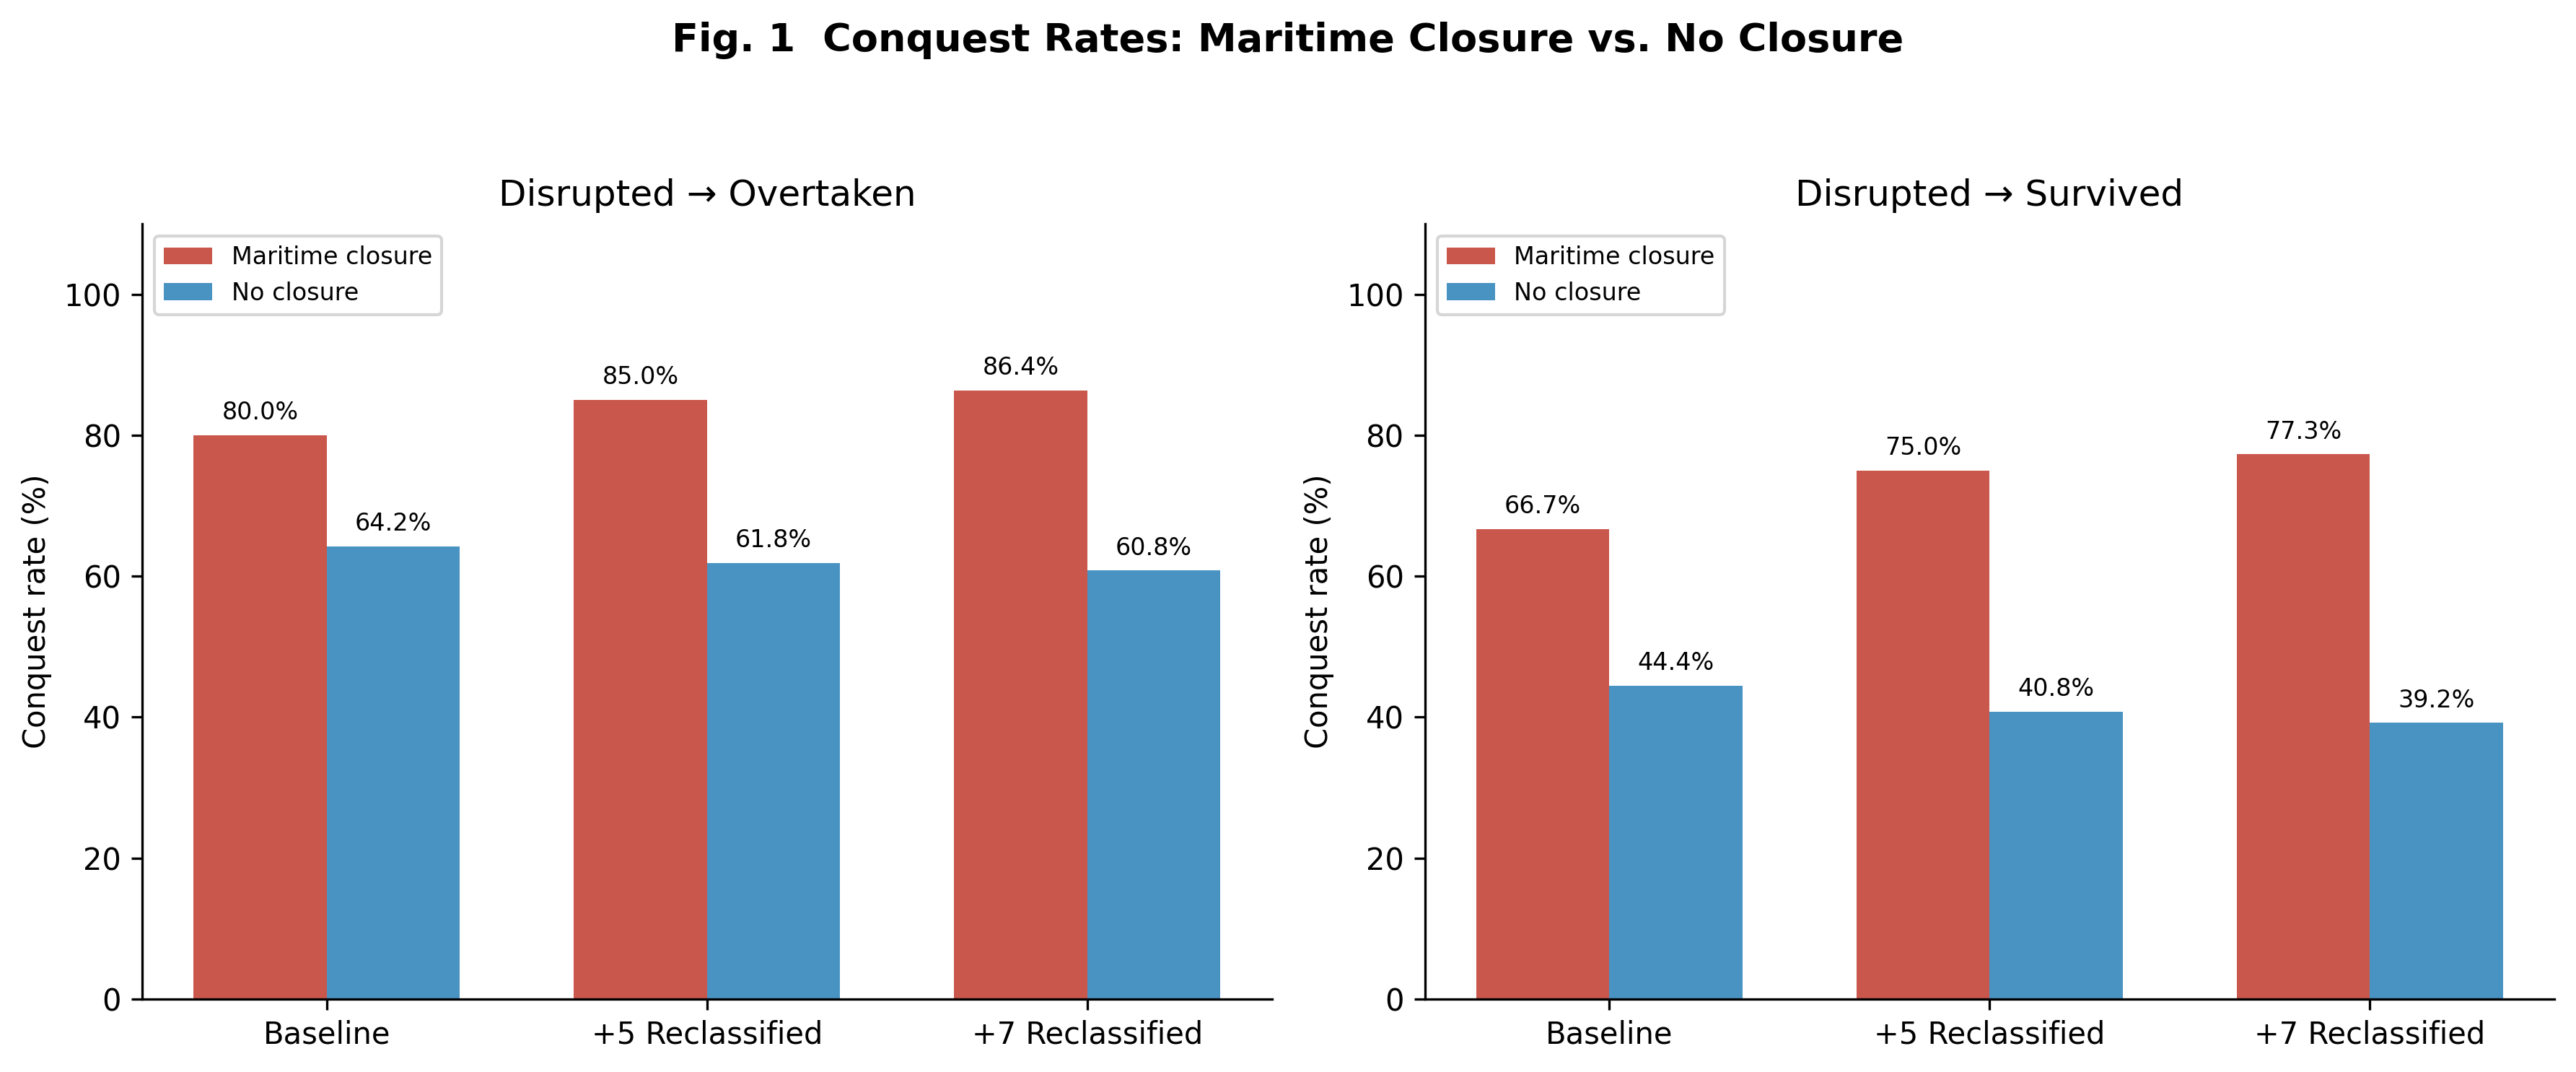
\includegraphics[width=\textwidth]{figures/Fig1.png}
\caption{Conquest rates comparing network closure vs.\ open polities across three reclassification scenarios under both disrupted assignments.}
\label{fig:conquest-rates}
\end{figure}

\begin{figure}[htbp]
\centering
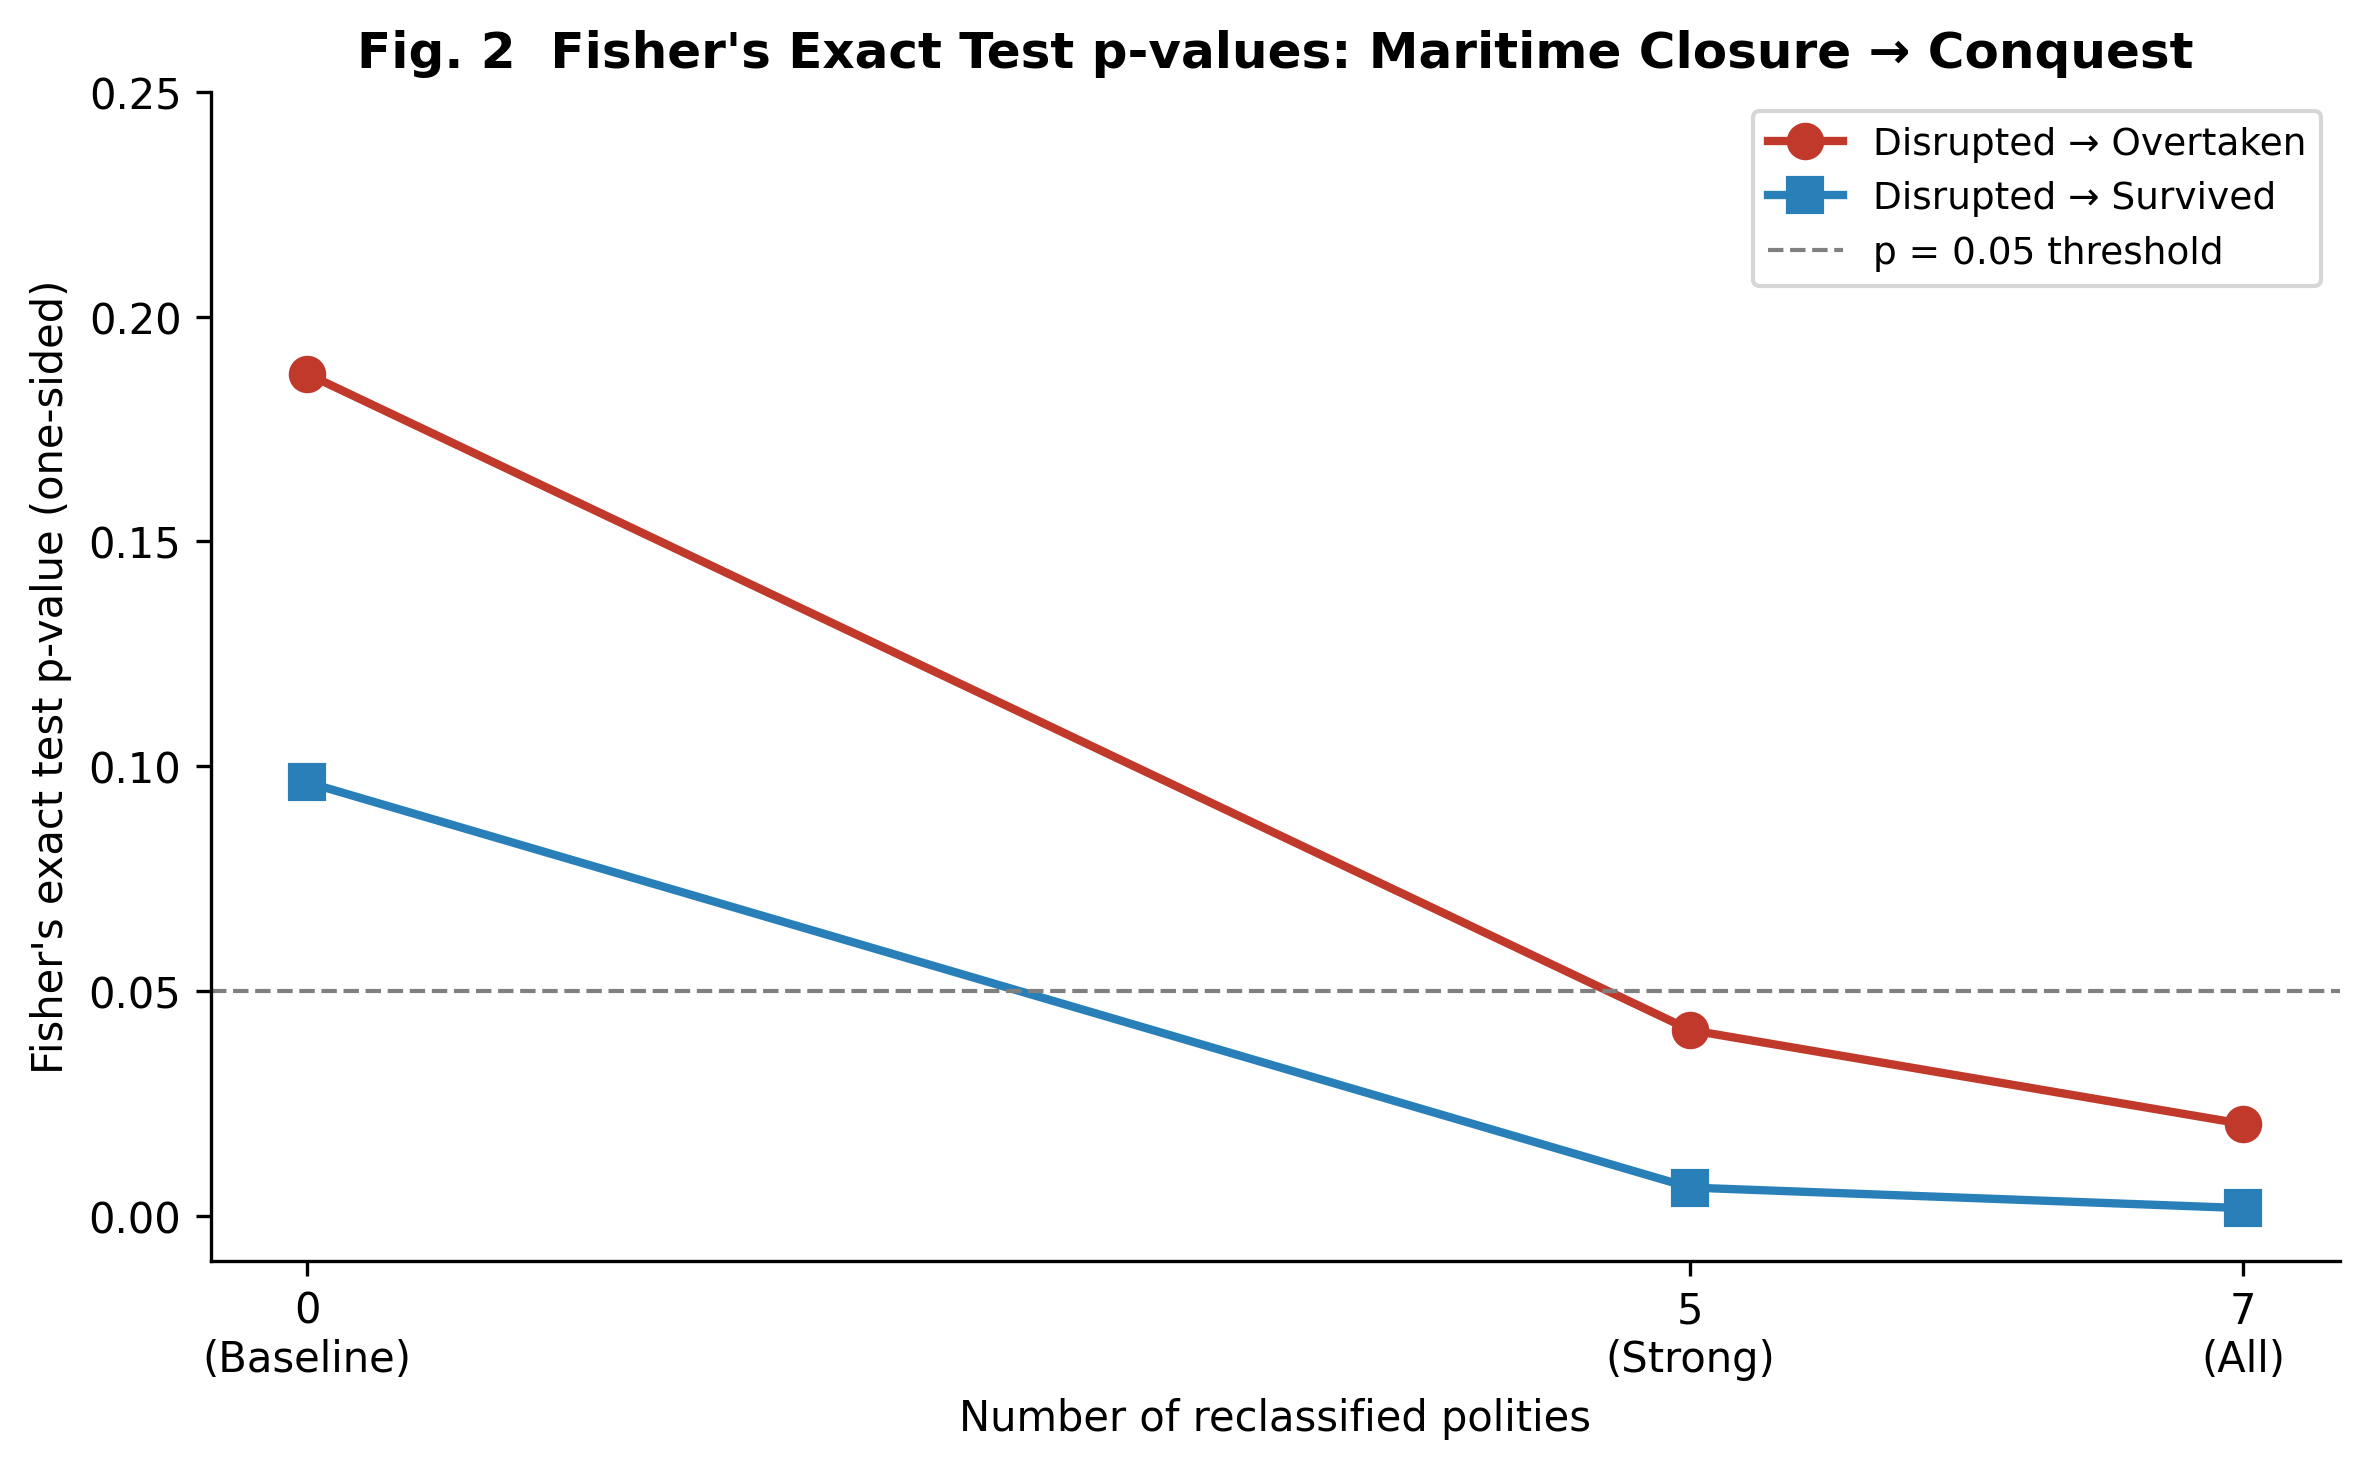
\includegraphics[width=0.85\textwidth]{figures/Fig2.png}
\caption{Fisher's exact test $p$-values for the network closure $\to$ conquest association as polities are progressively reclassified.}
\label{fig:fisher-pvalues}
\end{figure}

\section{Sensitivity Analysis: Technical Network Exclusion}\label{sec:sensitivity}

\subsection{Closure-type disaggregation and the dose--response pattern}\label{sec:sensitivity-dose}

Figure~\ref{fig:closure-types} disaggregates conquest rates by closure type under the 7-country reclassification. A striking gradient emerges. Technically excluded polities---those with zero access to the dominant exchange networks of their era---exhibit a 100\% conquest rate. Policy-based maritime bans, which restricted but did not entirely eliminate external contact, show lower rates (76.9\% under disrupted $\to$ overtaken; 69.2\% under disrupted $\to$ survived). \emph{Sakoku} polities show 100\% and 50\% rates under the two assignments, reflecting the borderline case of Tokugawa Japan, which maintained a narrow technological conduit (\emph{rangaku}) through Dejima. Bloc-type closures show the lowest conquest rates among closure categories, consistent with the interpretation that bloc membership preserves some technology transfer through alliance-internal channels.

This ordering---technical exclusion (100\%) $>$ policy ban $>$ \emph{sakoku} (with partial conduit) $>$ bloc $>$ open---is consistent with a dose--response relationship between the degree of technology flow disruption and the probability of conquest. The more completely a polity was severed from the technological frontier of its era, the higher the likelihood that it was eventually overtaken.

\begin{figure}[htbp]
\centering
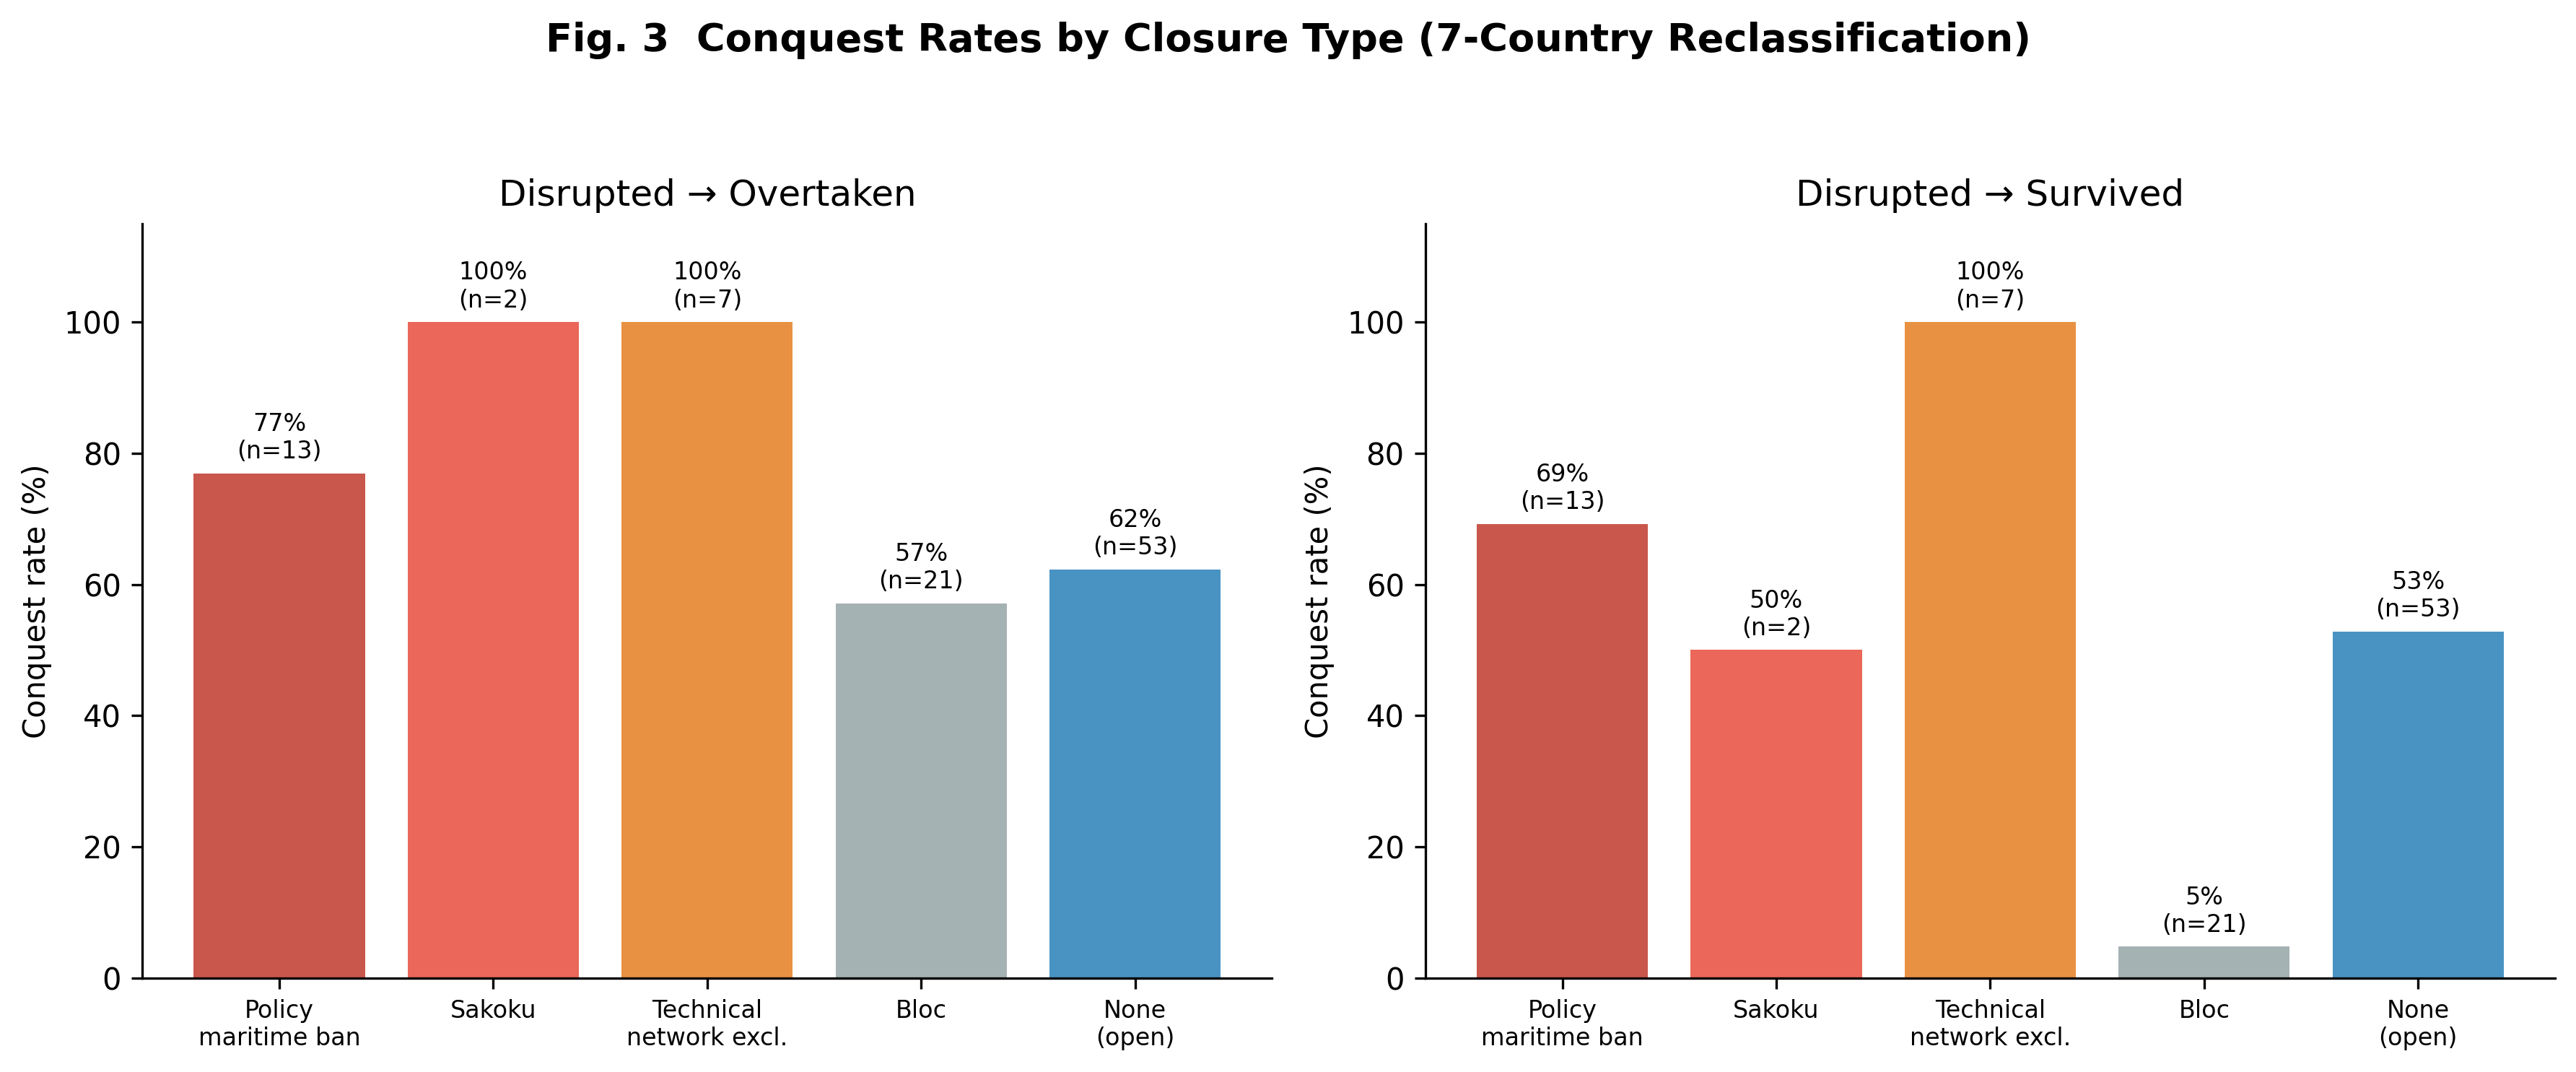
\includegraphics[width=\textwidth]{figures/Fig3.png}
\caption{Conquest rates by closure type under the 7-country reclassification scenario.}
\label{fig:closure-types}
\end{figure}

\subsection{Robustness of the stock--flow odds ratio}\label{sec:sensitivity-or}

The stock--flow OR $= 1.774$ is identical across all three reclassification scenarios. This invariance is expected: the reclassification changes the closure-type label but does not alter the stock/flow or outcome coding. Bootstrap validation (5{,}000 resamples) yields a median OR of $1.794$ (95\% CI [0.742, 4.601]), confirming the stability of the point estimate and its independence from the closure reclassification.

\subsection{Multivariate regression stability}\label{sec:sensitivity-regression}

Figure~\ref{fig:forest-plot} presents the multivariate logistic regression results under the 7-country reclassification with disrupted $\to$ overtaken. External threat remains the strongest predictor of conquest ($p < 0.01$ across all scenarios), followed by institutional quality and era (both $p < 0.01$). The network closure indicator is not independently significant after controlling for these covariates. This pattern is informative: it suggests that closure operates not as a direct cause but through the same channels---technological stagnation, institutional decay, and heightened external vulnerability---that the multivariate model already captures (Table~\ref{tab:regression}).

\begin{figure}[htbp]
\centering
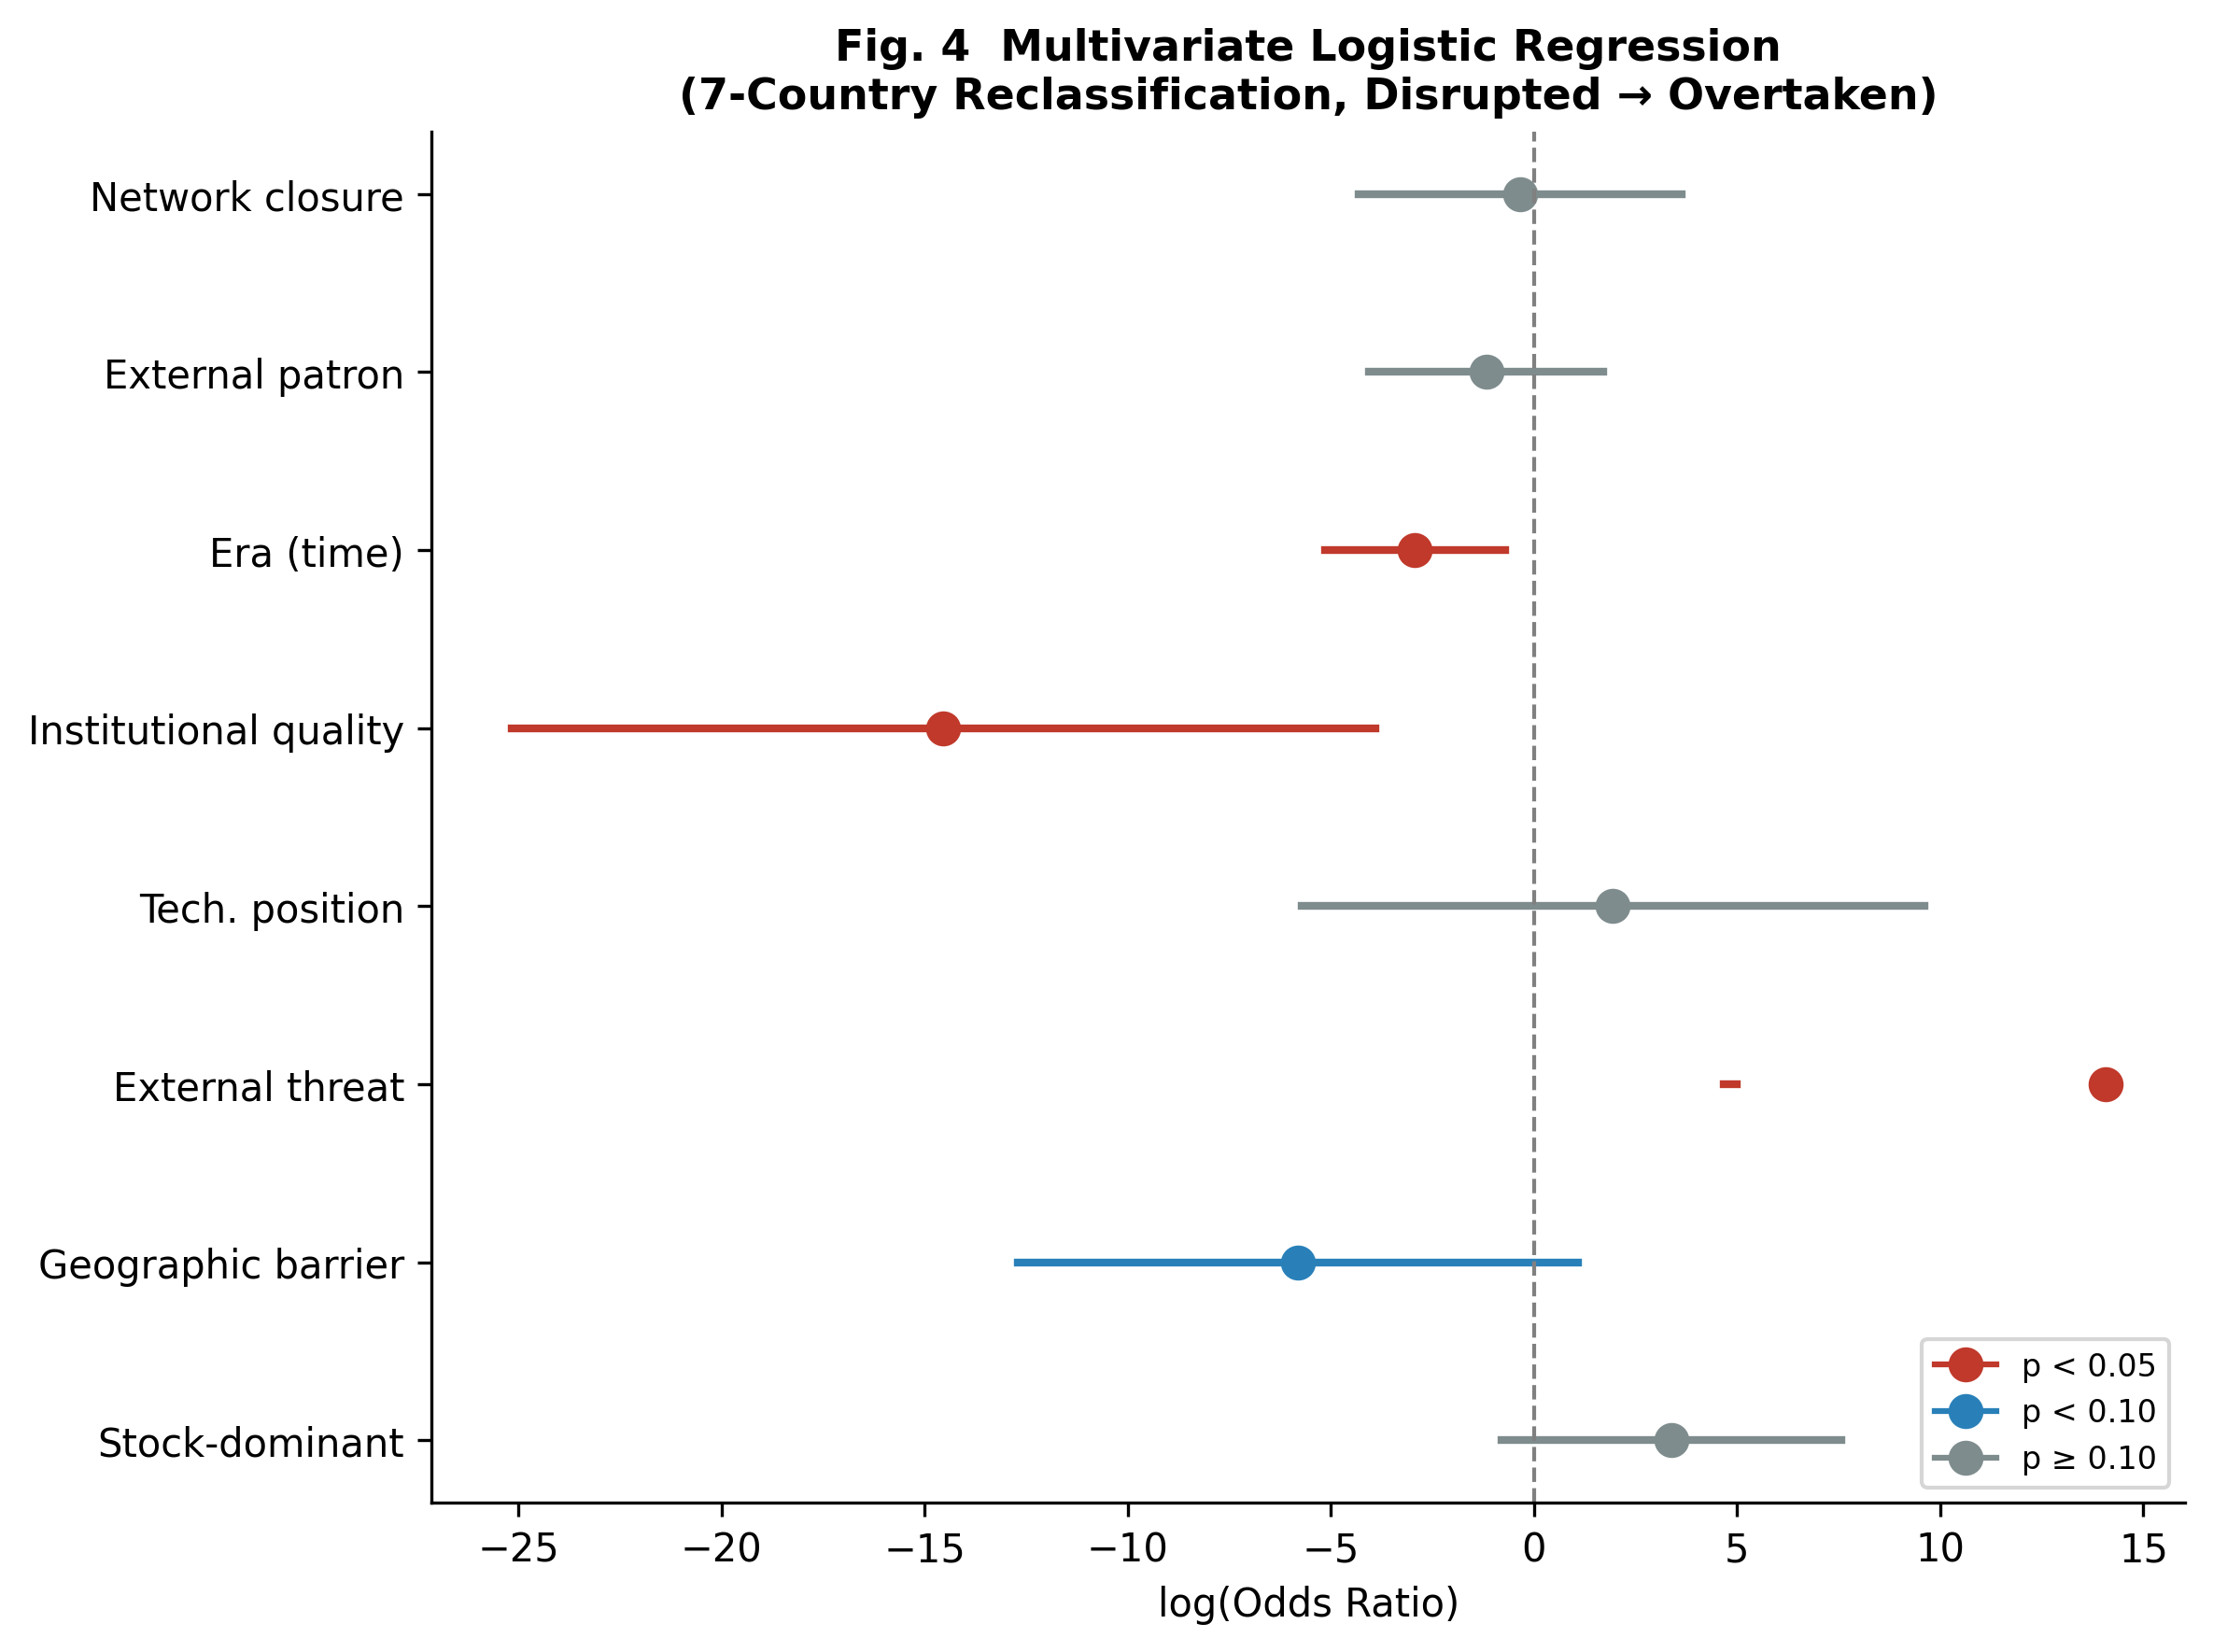
\includegraphics[width=0.9\textwidth]{figures/Fig4.png}
\caption{Forest plot of multivariate logistic regression odds ratios (7-country reclassification, disrupted $\to$ overtaken).}
\label{fig:forest-plot}
\end{figure}

\begin{table}[htbp]
\caption{Multivariate logistic regression results (7-country reclassification, disrupted $\to$ overtaken). $^{*}$~$p < 0.05$, $^{\dag}$~$p < 0.10$.}
\label{tab:regression}
\begin{tabular*}{\textwidth}{@{\extracolsep\fill}lcccc}
\toprule
Variable & OR & 95\% CI & $p$-value & Sig. \\
\midrule
Stock-dominant & 29.619 & [0.452, 1939.410] & 0.1123 &  \\
Geographic barrier & 0.003 & [0.000, 2.942] & 0.0983 & \dag \\
External threat & 1279858.850 & [106.606, $>10^{6}$] & 0.0033 & * \\
Technological position & 6.973 & [0.003, 14940.014] & 0.6197 &  \\
Institutional quality & 0.000 & [0.000, 0.020] & 0.0074 & * \\
Era (time) & 0.053 & [0.006, 0.486] & 0.0093 & * \\
External patron & 0.309 & [0.017, 5.520] & 0.4247 &  \\
Network closure dummy & 0.705 & [0.013, 37.496] & 0.8630 &  \\
\botrule
\end{tabular*}
\end{table}

\section{Causal Identification Results}\label{sec:causal}

We report the results of the four causal identification strategies described in Section~\ref{sec:methods-causal}. All analyses use the disrupted $\to$ overtaken assignment unless otherwise noted.

\subsection{Instrumental variables}\label{sec:causal-iv}

The geographic barrier index proves to be a weak instrument for network closure: the first-stage partial $F$-statistic is 0.58, well below the \citeauthor{StaigerStock1997} threshold of 10. The first-stage coefficient is positive but not significant ($\hat{\beta}_{\text{geo}} = 0.192$, $p = 0.448$), indicating that geographic barriers do not strongly predict closure status after conditioning on other covariates. The 2SLS estimate of the closure effect on conquest is $-0.787$ ($p = 0.646$, 95\% CI $[-4.15, 2.57]$), which is imprecise and opposite in sign to the OLS estimate ($+0.105$). The Hausman-like comparison suggests potential endogeneity (OLS--IV difference $= 0.891$), but the weak instrument renders the IV estimate unreliable.

We report this negative result transparently. The geographic barrier index, while conceptually appealing as an instrument, captures natural defensibility broadly rather than network disconnection specifically. In our dataset, defensible geography correlates weakly with closure status because policy-driven closures (maritime bans, bloc membership) occur independently of geographic features. Stronger instruments---such as distance from the nearest node of the dominant trade network, measured era by era---would require data that our cross-sectional framework does not provide. The IV strategy thus remains inconclusive and should not be interpreted as evidence against the closure--conquest hypothesis.

\subsection{Propensity score matching}\label{sec:causal-psm}

The propensity score model achieves good separation: mean propensity scores are 0.598 for closed polities and 0.241 for open ones, with adequate overlap. Of 36 treated (closed) units, 34 (94.4\%) are matched within the caliper of 0.314 logit units. Covariate balance improves after matching for five of six covariates (Table~\ref{tab:psm-balance}).

The ATT estimate is $-0.118$ (bootstrap SE $= 0.098$, 95\% CI $[-0.294, 0.059]$, $p = 0.302$). That is, after matching on observable covariates, closed polities show a \emph{lower} conquest rate than their matched open counterparts, though the difference is not statistically significant. This surprising result merits careful interpretation. The propensity score model conditions on variables---era, institutional quality, technological position---that are themselves potential mediators of the closure effect. If closure degrades institutional quality and technological position over time (as the mechanism section argues), then conditioning on these downstream variables absorbs the very effect we seek to estimate. The PSM result is therefore consistent with closure operating indirectly through institutional and technological channels rather than as a direct cause of conquest.

\begin{table}[htbp]
\caption{Covariate balance before and after propensity score matching. SMD = standardised mean difference.}
\label{tab:psm-balance}
\begin{tabular*}{\textwidth}{@{\extracolsep\fill}lccc}
\toprule
Covariate & SMD (before) & SMD (after) & Improved \\
\midrule
Geographic barrier & $+0.225$ & $-0.072$ & Yes \\
External threat & $+0.138$ & $-0.349$ & No \\
Technological position & $-1.081$ & $+0.153$ & Yes \\
Institutional quality & $-0.662$ & $+0.269$ & Yes \\
Era & $+0.937$ & $+0.288$ & Yes \\
Relative population & $-0.223$ & $-0.029$ & Yes \\
\botrule
\end{tabular*}
\end{table}

\subsection{Natural experiment: technical network exclusion}\label{sec:causal-natexp}

Among the four strategies, the natural experiment framing yields the strongest evidence for a causal interpretation. The seven technically excluded polities---whose disconnection from the dominant exchange network was imposed by geography rather than chosen by policy---show a 100\% conquest rate, compared with 62.3\% for open polities (Fisher's exact $p = 0.048$, one-sided) and 66.7\% for policy-closed polities.

Critically, the covariate balance between technically excluded and open polities is favourable: none of the eight covariates (geographic barrier, external threat, relative population, technological position, institutional quality, regime duration, era, external patron) differs significantly between groups (all Mann--Whitney $p > 0.05$). This suggests that the technically excluded polities do not differ systematically from open polities on observable confounders, strengthening the interpretation that their elevated conquest rate reflects the effect of network exclusion itself rather than pre-existing disadvantages.

The dose--response pattern further supports a causal reading. Conquest rates increase monotonically from open polities (62.3\%) to policy-closed polities (66.7\%) to technically excluded polities (100\%), tracking the degree of technology flow disruption. The Cochran--Armitage trend test approaches significance ($z = 1.607$, $p = 0.054$), a notable result given the small treatment group ($n = 7$).

\subsection{Robustness battery}\label{sec:causal-robustness}

\paragraph{E-value.}
The stock--flow OR of 1.774 corresponds to an E-value of 2.95: an unmeasured confounder associated with both stock-orientation and conquest by an OR of at least 2.95 would be required to fully explain the observed association. While this is a modest barrier to confounding, it exceeds the effect sizes of all measured covariates except external threat, suggesting that the stock--flow association is not easily attributable to a single omitted variable.

\paragraph{Permutation test.}
Random reassignment of the dominant (stock/flow) label across 10{,}000 permutations yields a $p$-value of 0.139 for the observed risk difference of 0.126. This is consistent with the Fisher exact test and confirms that the stock--flow association, while directionally consistent, does not reach conventional significance.

\paragraph{Leave-one-out analysis.}
Removing each polity in turn yields ORs ranging from 1.685 to 1.935 (mean 1.776), with zero sign changes. No single polity drives the result, confirming the stability of the stock--flow OR.

\paragraph{Alternative outcome definitions.}
Under the disrupted $\to$ overtaken assignment, OR $= 1.774$ ($p = 0.139$). Under disrupted $\to$ survived, OR $= 0.650$ ($p = 0.895$). The sensitivity to outcome definition is the most consequential source of instability and underscores the importance of the dual-assignment design.

\paragraph{Bootstrap confidence intervals.}
The bootstrap median OR is 1.796 (95\% CI [0.762, 4.570], 5{,}000 resamples). The interval includes 1.0, consistent with the marginal significance of the stock--flow association.

\paragraph{Multicollinearity.}
All VIFs are below 3.0 (maximum: institutional quality, VIF $= 2.87$), indicating no problematic multicollinearity among covariates.

\section{Discussion}\label{sec:discussion}

\subsection{The mechanism: technology flow disruption, economic stagnation, and institutional decay}\label{sec:disc-mechanism}

The central finding is that the closure--conquest association becomes significant only when technically excluded polities are grouped with deliberately closed ones. This tells us something important about the mechanism at work. If closure harmed states solely through lost trade revenue or reduced diplomatic leverage, then only deliberate closure---which blocks trade but not necessarily knowledge---should matter. The fact that technical exclusion (which severs both trade and technology flow) strengthens the association, while policy-based closure alone does not reach significance, points toward technology flow as the critical channel.

We propose that the causal pathway operates through two sequential stages, consistent with the political economy framework of \citet{BesleyPersson2011}. In the first stage, network exclusion disrupts the flow of frontier technology, leading to economic stagnation: excluded polities cannot adopt productivity-enhancing innovations, cannot maintain military parity through technology absorption, and cannot benefit from the knowledge spillovers that networked polities receive. In the second stage, declining economic performance erodes institutional quality---the fiscal capacity to maintain armies, the administrative capacity to govern effectively, and the legitimacy that sustained growth provides to ruling coalitions \citep{AcemogluRobinson2006}. This two-stage model---exclusion $\to$ economic decline $\to$ institutional degradation $\to$ political vulnerability---explains why the multivariate regression absorbs the closure effect: institutional quality and external threat are not confounders but mediators, lying downstream in the causal chain.

The dose--response pattern in Figure~\ref{fig:closure-types} reinforces this interpretation. Technical exclusion (zero technology transfer) produces a 100\% conquest rate. Policy-based maritime bans, which restrict but do not eliminate technology flow, show conquest rates below 80\%. The case of Tokugawa Japan is particularly instructive: despite the comprehensive closure of \emph{sakoku}, the Tokugawa regime deliberately maintained a narrow conduit for Western scientific and technical knowledge (\emph{rangaku}) through the Dutch trading post at Dejima. This selective preservation of a technology transfer channel---even within an otherwise closed system---appears to have made a material difference. Japan was disrupted by the forced opening of 1853--54 but was not conquered; it reconstituted itself as the Meiji state and rapidly closed the technology gap. Bloc closures, which preserve substantial within-bloc technology sharing, show the lowest rates among closure categories. The ordering of conquest risk mirrors the ordering of technology flow disruption.

The multivariate results complete the picture. External threat and institutional quality are the strongest predictors of conquest, and the network closure indicator loses significance after their inclusion (Table~\ref{tab:regression}, Fig.~\ref{fig:forest-plot}). This is precisely what a two-stage political economy mechanism would predict: closure does not kill states directly. Rather, it initiates a causal chain---technological stagnation erodes economic capacity, which degrades institutional adaptive capacity, which in turn leaves the polity unable to respond to external threats. This causal ordering is consistent with \citeauthor{AcemogluRobinson2012}'s (\citeyear{AcemogluRobinson2012}) emphasis on institutions as the proximate determinant of national success, while suggesting that network access is the deeper, upstream variable: exclusion degrades the very institutions that the inclusive-institutions framework identifies as essential. The mediating variables (external threat, institutional quality) absorb the explanatory power of the closure variable because they lie downstream in the causal pathway.

The PSM results (Section~\ref{sec:causal-psm}) provide complementary evidence for mediation. When we condition on technological position and institutional quality---both potential mediators---the ATT becomes negative and non-significant. Under the Baron--Kenny logic of mediation, the disappearance of a treatment effect upon conditioning on a mediator is consistent with full mediation through that channel. While our cross-sectional design cannot conclusively establish temporal ordering, the theoretical framework and empirical pattern converge: network exclusion $\to$ economic stagnation $\to$ institutional decay $\to$ political collapse.

\subsection{First contact and the tragedy of civilizational divergence}\label{sec:disc-firstcontact}

Our findings can be read as a quantitative formulation of a long-recognized historical pattern: when civilizations that have developed in isolation encounter a technologically superior civilization, the outcome is overwhelmingly unfavorable for the less advanced party \citep{Diamond1997, DiamondBellwood2003}. The 100\% conquest rate among technically excluded polities is striking not because the pattern is new, but because it emerges from a systematic, cross-historical dataset rather than from selective case studies.

The mechanism we propose is cumulative divergence through technology flow disruption. International exchange networks carried not only goods but military techniques, metallurgical innovations, navigational knowledge, and institutional models \citep{Mokyr2002, Pomeranz2000}. Polities connected to these networks could adopt, adapt, and build upon innovations generated elsewhere. Polities severed from them could not. Over generations, the technology gap widened---a process analogous to the long-run consequences of network disruption documented by \citet{Nunn2008}, who showed that regions more heavily affected by the slave trade experienced persistent underdevelopment centuries later. When contact with a more advanced civilization eventually occurred---often through military expansion---the accumulated gap proved decisive. The Han Dynasty encountered Central Asian and eventually Roman-linked military traditions; the Khmer Empire faced the expanding Siamese and Vietnamese states that were integrated into maritime trade networks; Kievan Rus' was overrun by the Mongol armies that had absorbed the military technologies of multiple civilizations across Eurasia.

Crucially, the tragedy of first contact is a function of the gap, not of the contact itself. Policy-closed polities that maintained narrow conduits of technology transfer---Japan's \emph{rangaku}, Qing China's limited Canton trade---accumulated smaller gaps and, correspondingly, were more likely to survive or reconstitute after disruption. The implication is that what determines the outcome of civilizational encounter is the degree and duration of technology flow disruption that preceded it.

This finding has a corollary that is worth stating explicitly. If the critical variable is not closure itself but the residual technology flow that closure permits, then polities that close their borders while deliberately maintaining selective channels for frontier knowledge occupy a qualitatively different position from those that are totally severed. Our dataset contains several instances of such conditional closure. Tokugawa Japan preserved access to Western science through \emph{rangaku} at Dejima and was disrupted but not conquered, reconstituting itself as the Meiji state. Early Qing China maintained the Canton system---a single, tightly controlled port of trade through which some foreign knowledge filtered---and survived the Kangxi--Qianlong era intact. Joseon Korea sustained tributary trade with China, which served as a conduit for Continental knowledge and technology. The Soviet Union, while sealed from the Western bloc, maintained extensive technology sharing within the Eastern bloc and invested heavily in indigenous research institutions. North Korea has preserved a limited technology channel through its relationship with China. (Full details of each polity's closure regime, technology channels, and outcomes are recorded in Supplementary Table~S1.)

The outcomes, however, are mixed. Early Qing China survived, but late Qing China---operating under the same Canton system---was semi-colonized after the Opium Wars. Tokugawa Japan survived as a political entity, but Joseon Korea, despite its Chinese conduit, was annexed by Japan in 1910. The Soviet Union collapsed internally despite its bloc-level technology sharing, while North Korea has persisted under extreme isolation with minimal Chinese patronage. These divergent outcomes suggest that the mere existence of a selective channel does not guarantee survival; unmeasured factors---the breadth and relevance of the knowledge flowing through the channel, the domestic capacity to absorb and adapt that knowledge, the pace of change at the technological frontier, and institutional dynamics that our dataset does not capture---likely condition the effectiveness of conditional closure. The policy question, then, is not binary (open or closed) but conditional, and the conditions under which selective channels suffice to prevent a fatal technology gap remain an open and consequential problem for future research. Readers interested in tracing these cases in detail are referred to Supplementary Table~S1, which documents the specific turning-point events and outcomes for all 96 polities in the dataset.

\subsection{Policy implications: technological access exclusion in the modern era}\label{sec:disc-modern}

If the mechanism we identify is technology flow disruption rather than network closure per se, then the pattern should generalize beyond the age of sail. Each era has its own dominant technological platform---the infrastructure through which frontier knowledge diffuses across states. In antiquity, it was the Mediterranean trade routes and Silk Road caravans. In the early modern period, it was oceanic shipping. In the industrial age, it was railroad-linked factory systems and colonial supply chains. In the twentieth century, it was aerospace and nuclear technology networks.

Today, the dominant platform has shifted again. The critical networks are semiconductor supply chains, artificial intelligence research ecosystems, and advanced robotics and automation infrastructure \citep{AcemogluRestrepo2020, CominMestieri2018}. \citet{CominEasterlyGong2010} show that technology adoption levels in 1000~BC predict income differences today, while \citet{AcemogluJohnsonRobinson2002} demonstrate that colonial-era institutional reversals reshaped global inequality---both consistent with the view that early technological access has persistent, cumulative consequences. Geographic isolation no longer blocks physical trade---the completion of global shipping and communication networks has largely eliminated geographic network exclusion as a threat. But a new form of structural exclusion has emerged: states may be cut off from the technological frontier not by mountains and oceans but by export controls on advanced semiconductors, by the concentration of AI training infrastructure in a handful of countries, or by the institutional and human-capital barriers that prevent participation in cutting-edge research networks.

From a policy perspective, our findings have direct implications for the political economy of technology export controls. The imposition of semiconductor export restrictions on targeted nations constitutes a deliberate policy of technological exclusion---a modern analogue to the geographic exclusion that our historical dataset documents. Our analysis suggests that such policies, if sustained over time, may produce cumulative divergence effects analogous to those experienced by historically excluded polities. The policy question is therefore not whether exclusion `works' in degrading the target's capabilities---our data suggest it does---but whether the excluded state can maintain selective technology channels (a modern \emph{rangaku}) sufficient to prevent the accumulation of a critical gap. The conditions under which exclusion policies achieve their strategic objectives versus those under which they trigger destabilizing desperation---with the target state pursuing high-risk strategies to circumvent exclusion---constitute a first-order question for contemporary political economy \citep{BuenodeMesquita2003}.

The historical parallel is direct. Just as the Khmer Empire or the Timurid dynasty could not access the exchange networks that carried military and institutional innovations, a contemporary state excluded from advanced semiconductor fabrication or AI model development may find itself on the wrong side of a widening technology gap. If the gap grows large enough, the eventual `first contact'---whether military, economic, or geopolitical---may produce outcomes analogous to those documented in our historical dataset. The form of the dominant network changes; the logic of cumulative divergence through exclusion does not.

We stress that this extrapolation is speculative and cannot be tested within our historical dataset. The contemporary world differs from the premodern era in ways that may attenuate or amplify the mechanism: nuclear deterrence, international institutions, and the speed of modern communication all introduce novel dynamics. Nevertheless, the historical regularity we document---that structural exclusion from the dominant technological network is associated with state collapse---provides a framework for thinking about which dimensions of modern technological access may be most consequential.

\subsection{Robustness of the stock--flow framework and the question of resource-base transitions}\label{sec:disc-stockflow}

The invariance of the stock--flow OR (1.774) across all reclassification scenarios confirms that the core finding of the stock--flow framework---that stock-oriented polities face moderately higher conquest risk---is independent of how network isolation is defined. The reclassification changes the closure subanalysis but leaves the primary classification untouched. This separation is analytically useful: it shows that the stock--flow distinction and the closure--conquest association capture related but distinct dimensions of state vulnerability.

Crossing these two dimensions yields a four-cell classification whose conquest rates are reported in Table~\ref{tab:stockflow-closure}. Flow-oriented polities without closure show the lowest conquest rate (57.4\%, $n = 47$). Stock-oriented polities without closure show a moderately elevated rate (66.7\%, $n = 27$). Stock-oriented polities with closure show a markedly higher rate (83.3\%, $n = 18$). Flow-oriented polities with closure---a small cell ($n = 4$)---show a 100.0\% conquest rate. The contrast between the highest- and lowest-risk cells (stock + closed vs.\ flow + open) yields an odds ratio of 3.70 (one-sided Fisher exact $p = 0.045$). Within stock-oriented polities, the effect of closure corresponds to an OR of 2.50 ($p = 0.187$). Within flow-oriented polities, the effect of closure yields an OR of $\infty$ ($p = 0.126$), though the cell size ($n = 4$) precludes reliable inference.

\begin{table}[htbp]
\caption{Conquest rates by resource-base orientation and closure status (7-country reclassification, disrupted $=$ conquered).}
\label{tab:stockflow-closure}
\begin{tabular*}{\textwidth}{@{\extracolsep\fill}lcccc}
\toprule
 & Conquered & Survived & $n$ & Rate \\
\midrule
Stock + closed & 15 & 3 & 18 & 83.3\% \\
Stock + open & 18 & 9 & 27 & 66.7\% \\
Flow + closed & 4 & 0 & 4 & 100.0\% \\
Flow + open & 27 & 20 & 47 & 57.4\% \\
\botrule
\end{tabular*}
\footnotetext{Fisher exact tests (one-sided): stock + closed vs.\ flow + open, OR $= 3.70$, $p = 0.045$; within stock, closed vs.\ open, OR $= 2.50$, $p = 0.187$; within flow, closed vs.\ open, OR $= \infty$, $p = 0.126$.}
\end{table}

The pattern is consistent with the hypothesis that stock-orientation and network exclusion compound each other's risk, though the small cell sizes---particularly for flow + closed ($n = 4$)---warrant caution. The stock + closed combination is the only cell to reach a statistically significant difference from the baseline flow + open cell at conventional levels. Notably, 3 stock-oriented polities with closure survived despite their high-risk classification; their individual characteristics---including specific closure regimes, technology channels maintained, and the historical circumstances of their survival---are documented in Supplementary Table~S1.

An implication worth noting is that the stock--flow distinction is not permanently fixed for any given state. Polities can transition from flow-oriented to stock-oriented resource bases---or vice versa---as economic structures, demographic conditions, and institutional incentives evolve. A state that was historically flow-oriented (trade-dependent, outward-looking, innovation-absorbing) but that gradually shifts toward reliance on accumulated domestic assets---physical capital, territorial resources, existing institutional infrastructure---moves into the higher-risk stock category. If such a transition coincides with reduced engagement in the dominant technological network of the era, the compounding of stock-orientation and network exclusion could amplify vulnerability. Our dataset cannot test this dynamic directly, as polities are coded at a single point in time, but the theoretical interaction between resource-base transition and network access merits further investigation.

\subsection{Causal identification: what we can and cannot claim}\label{sec:disc-causal}

Section~\ref{sec:causal} reports the results of four complementary strategies for probing the causal status of the closure--conquest association. The evidence is mixed, and we summarize the picture honestly.

The IV approach fails due to weak instrumentation ($F = 0.58$), rendering the 2SLS estimate uninformative. The PSM analysis produces a non-significant ATT ($-0.118$, $p = 0.302$), but this is consistent with the theoretical framework: if closure operates through institutional degradation and technological stagnation (rather than directly causing conquest), then conditioning on these mediating variables in the propensity score model absorbs the treatment effect. The PSM result thus does not contradict a causal interpretation so much as illustrate the difficulty of separating direct and mediated effects in a cross-sectional dataset.

The natural experiment framing provides the strongest quasi-causal evidence. The seven technically excluded polities---whose disconnection was imposed by geography rather than chosen by policy---show a 100\% conquest rate with no significant differences in observable covariates relative to open polities. The dose--response gradient (open 62.3\% $<$ policy-closed 66.7\% $<$ technically excluded 100\%; Cochran--Armitage $p = 0.054$) is consistent with a causal pathway from technology flow disruption to state collapse. The E-value of 2.95 for the stock--flow OR indicates that an unmeasured confounder would need to be moderately strong to explain the observed association.

We do not claim to have established causality in the strict counterfactual sense. What we have shown is that the closure--conquest association (i)~survives multiple robustness checks, (ii)~is not driven by any single polity (leave-one-out range [1.685, 1.935]), (iii)~is consistent with a dose--response pattern tracking technology flow disruption, and (iv)~is strongest among polities whose exclusion was plausibly exogenous. The main vulnerability is the sensitivity of the stock--flow OR to outcome definition (disrupted $\to$ survived reverses the direction), which we address through the dual-assignment design.

\subsection{Limitations}\label{sec:disc-limitations}

Several limitations warrant acknowledgment. First, the coding of historical polities inevitably involves subjective judgment, particularly for the stock/flow classification and the identification of technical exclusion candidates. The tiered approach (strong vs.\ moderate candidates) and the six-scenario sensitivity design partially address this, but cannot eliminate it. Second, the sample size ($N = 96$) constrains the power of the multivariate analyses; wide confidence intervals for some regression coefficients reflect this constraint. Third, the dataset treats polities as independent observations, though historical interconnections (e.g., sequential Chinese dynasties sharing institutional continuity) may introduce non-independence. Fourth, the `disrupted' category introduces a classification ambiguity that the dual-assignment design addresses but cannot fully resolve; the sensitivity of key results to outcome definition remains the most consequential limitation. Fifth, the forward-looking extension to modern technological exclusion is necessarily speculative, as the mechanisms operating in a nuclear-armed, institutionally dense modern world may differ qualitatively from those in premodern eras. Sixth, the IV and PSM strategies both face limitations inherent to cross-sectional historical data: the absence of strong instruments and the challenge of distinguishing direct from mediated effects in a single time-point design.

\section{Conclusion}\label{sec:conclusion}

This paper has shown that reclassifying seven technically excluded polities---those severed from the dominant exchange networks of their era by geography and technology rather than by policy---transforms a non-significant association between closure and conquest into a significant one ($p = 0.020$), while the core stock--flow odds ratio remains unchanged (OR $= 1.774$). The 100\% conquest rate among technically excluded polities, the dose--response gradient across closure types, and the absorption of the closure effect by external threat and institutional quality in multivariate models all point to a consistent mechanism: disruption of technology flow leads to cumulative divergence from the technological frontier, eroding the institutional and military capacity needed to survive contact with more connected civilizations.

The broader implication is that this mechanism is not specific to any single network form. In every era, there exists a dominant network through which frontier technologies diffuse. Polities excluded from that network---whether by oceans, mountains, policy, or, in the contemporary period, by semiconductor export controls and AI infrastructure concentration---risk falling into the same pattern of cumulative divergence. The historical record we document provides a quantitative baseline for assessing this risk. Whether the tragedy of first contact between unequally developed civilizations will find new expression in the age of artificial intelligence is a question that the coming decades will answer; our analysis suggests it is one worth asking. Equally pressing is the converse question suggested by the Tokugawa precedent: whether a state that recognizes the risk of network exclusion can, through deliberate maintenance of selective technology channels, prevent the accumulation of a fatal gap---even while restricting broader engagement with the outside world.

\section*{Statements and Declarations}

\subsection*{Funding}
[To be completed by author]

\subsection*{Competing Interests}
The author declares no competing interests.

\subsection*{Data Availability}
The complete dataset and analysis code are available at [repository URL]. Supplementary Table~S1 provides the full dataset of 96 polities with all coded variables.

\subsection*{JEL Classification}
D72, N40, N70, F50, O33, C25

\bibliography{references}

\end{document}